\documentclass[tikz,border=5pt]{standalone}
\usepackage{amsmath}
\usetikzlibrary{arrows.meta}

\tikzset{
  vertex/.style={
    circle,
    draw,
    semithick,
    inner sep=0pt,
    minimum size=5.5mm,
    font=\small
  },
  edge/.style={-{Stealth[length=2mm]},semithick},
  relation/.style={font=\small,align=center},
  note/.style={font=\scriptsize,align=center}
}

\begin{document}
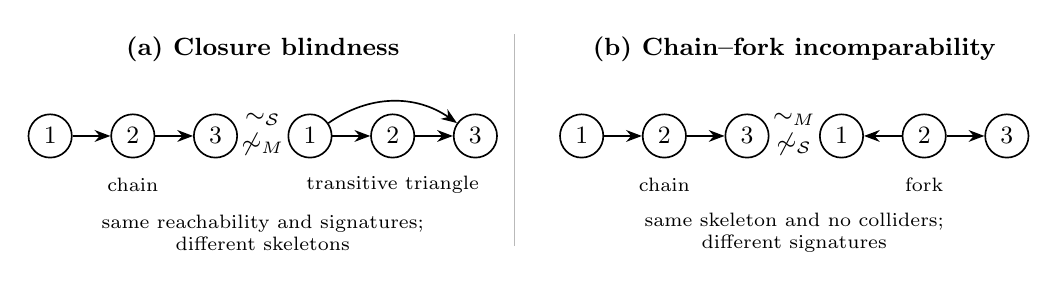
\begin{tikzpicture}[x=1cm,y=1cm]
  % Panel (a): identical path signatures, different Markov classes.
  \node[font=\small\bfseries] at (3.15,2.55)
    {(a) Closure blindness};

  \node[vertex] (a1) at (0.45,1.45) {1};
  \node[vertex] (a2) at (1.50,1.45) {2};
  \node[vertex] (a3) at (2.55,1.45) {3};
  \draw[edge] (a1) -- (a2);
  \draw[edge] (a2) -- (a3);
  \node[note] at (1.50,0.83) {chain};

  \node[relation] at (3.15,1.47)
    {$\sim_{\mathcal S}$\\[-1pt]$\not\sim_M$};

  \node[vertex] (b1) at (3.75,1.45) {1};
  \node[vertex] (b2) at (4.80,1.45) {2};
  \node[vertex] (b3) at (5.85,1.45) {3};
  \draw[edge] (b1) -- (b2);
  \draw[edge] (b2) -- (b3);
  \draw[edge] (b1) to[bend left=35] (b3);
  \node[note] at (4.80,0.83) {transitive triangle};

  \node[note] at (3.15,0.22)
    {same reachability and signatures;\\different skeletons};

  % Divider.
  \draw[gray!55] (6.35,0.05) -- (6.35,2.75);

  % Panel (b): identical Markov classes, different path signatures.
  \begin{scope}[xshift=6.75cm]
    \node[font=\small\bfseries] at (3.15,2.55)
      {(b) Chain--fork incomparability};

    \node[vertex] (c1) at (0.45,1.45) {1};
    \node[vertex] (c2) at (1.50,1.45) {2};
    \node[vertex] (c3) at (2.55,1.45) {3};
    \draw[edge] (c1) -- (c2);
    \draw[edge] (c2) -- (c3);
    \node[note] at (1.50,0.83) {chain};

    \node[relation] at (3.15,1.47)
      {$\sim_M$\\[-1pt]$\not\sim_{\mathcal S}$};

    \node[vertex] (d1) at (3.75,1.45) {1};
    \node[vertex] (d2) at (4.80,1.45) {2};
    \node[vertex] (d3) at (5.85,1.45) {3};
    \draw[edge] (d2) -- (d1);
    \draw[edge] (d2) -- (d3);
    \node[note] at (4.80,0.83) {fork};

    \node[note] at (3.15,0.22)
      {same skeleton and no colliders;\\different signatures};
  \end{scope}
\end{tikzpicture}
\end{document}
